\begin{figure}[ht]
    \centering
    \subfloat[]{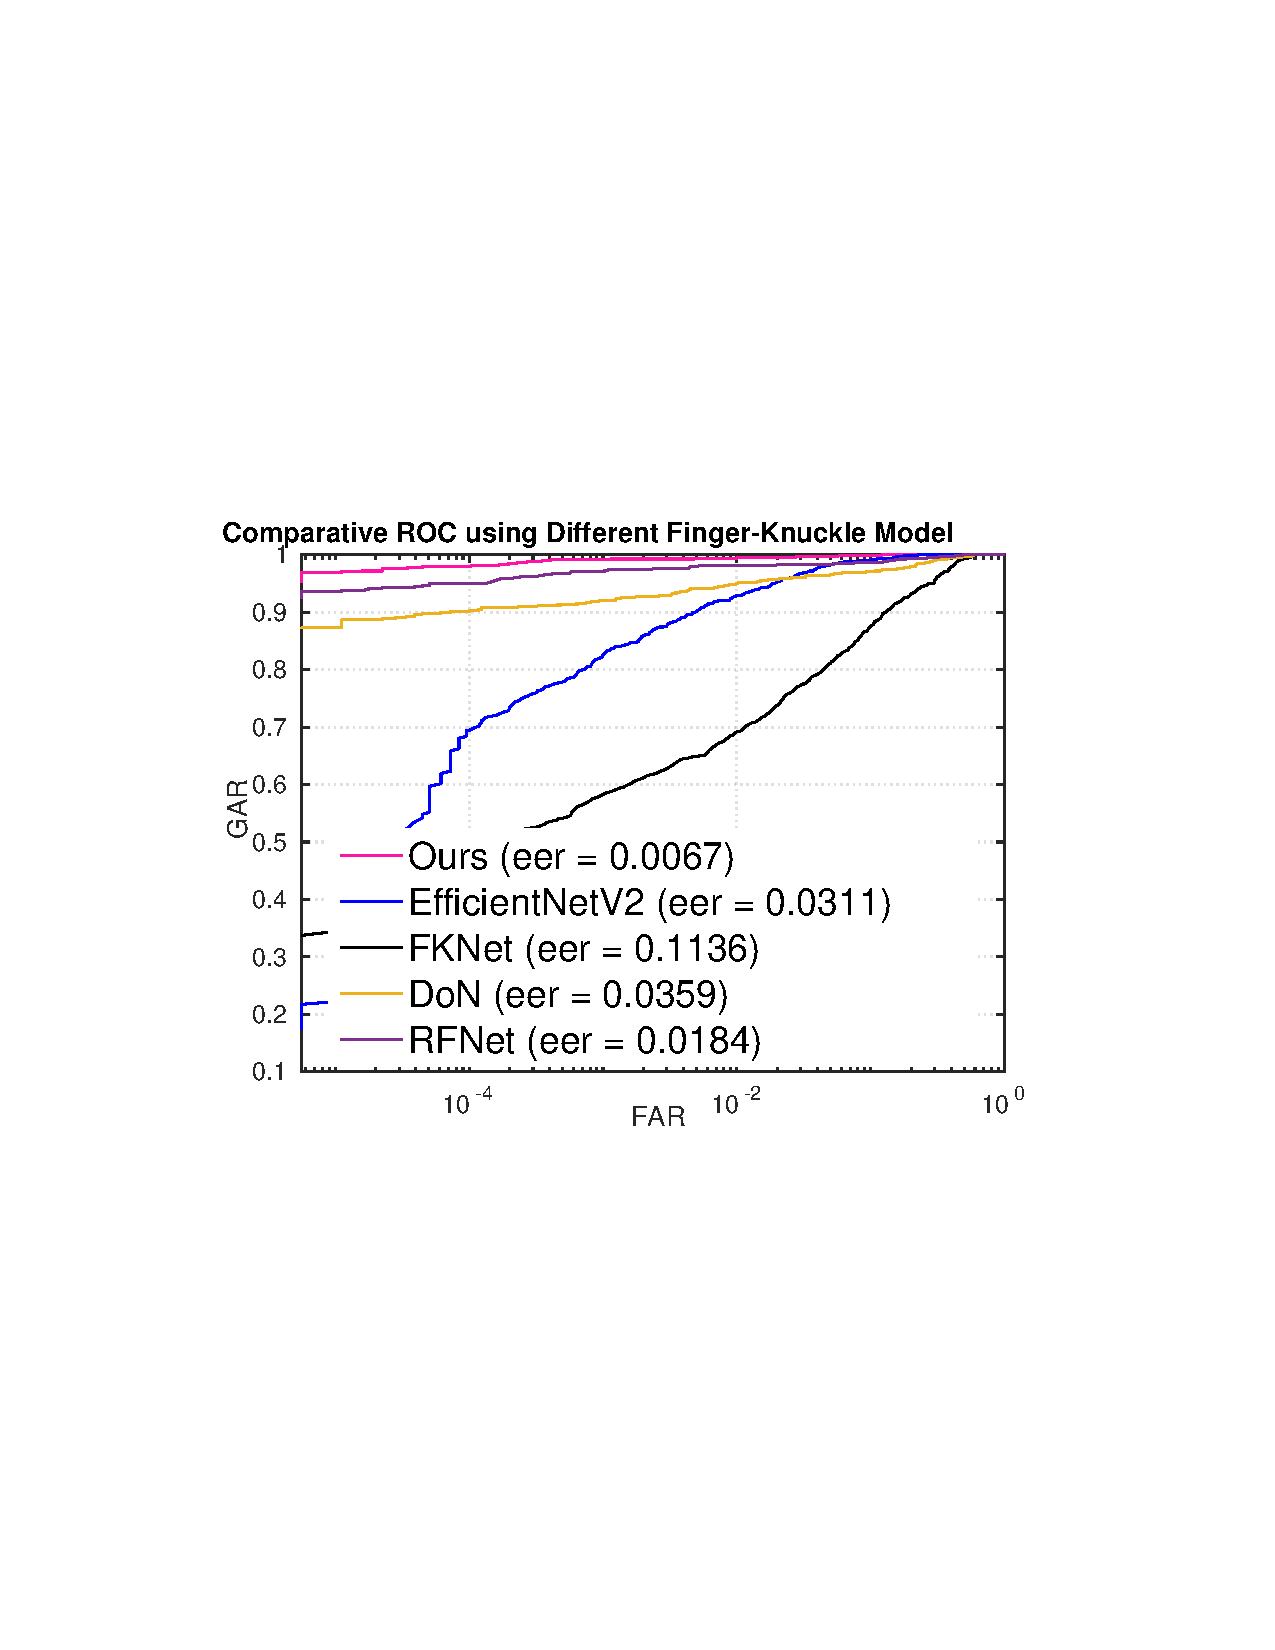
\includegraphics[width=1.6in]{Figures/fk-compare/02.pdf}
    \label{}}
    \subfloat[]{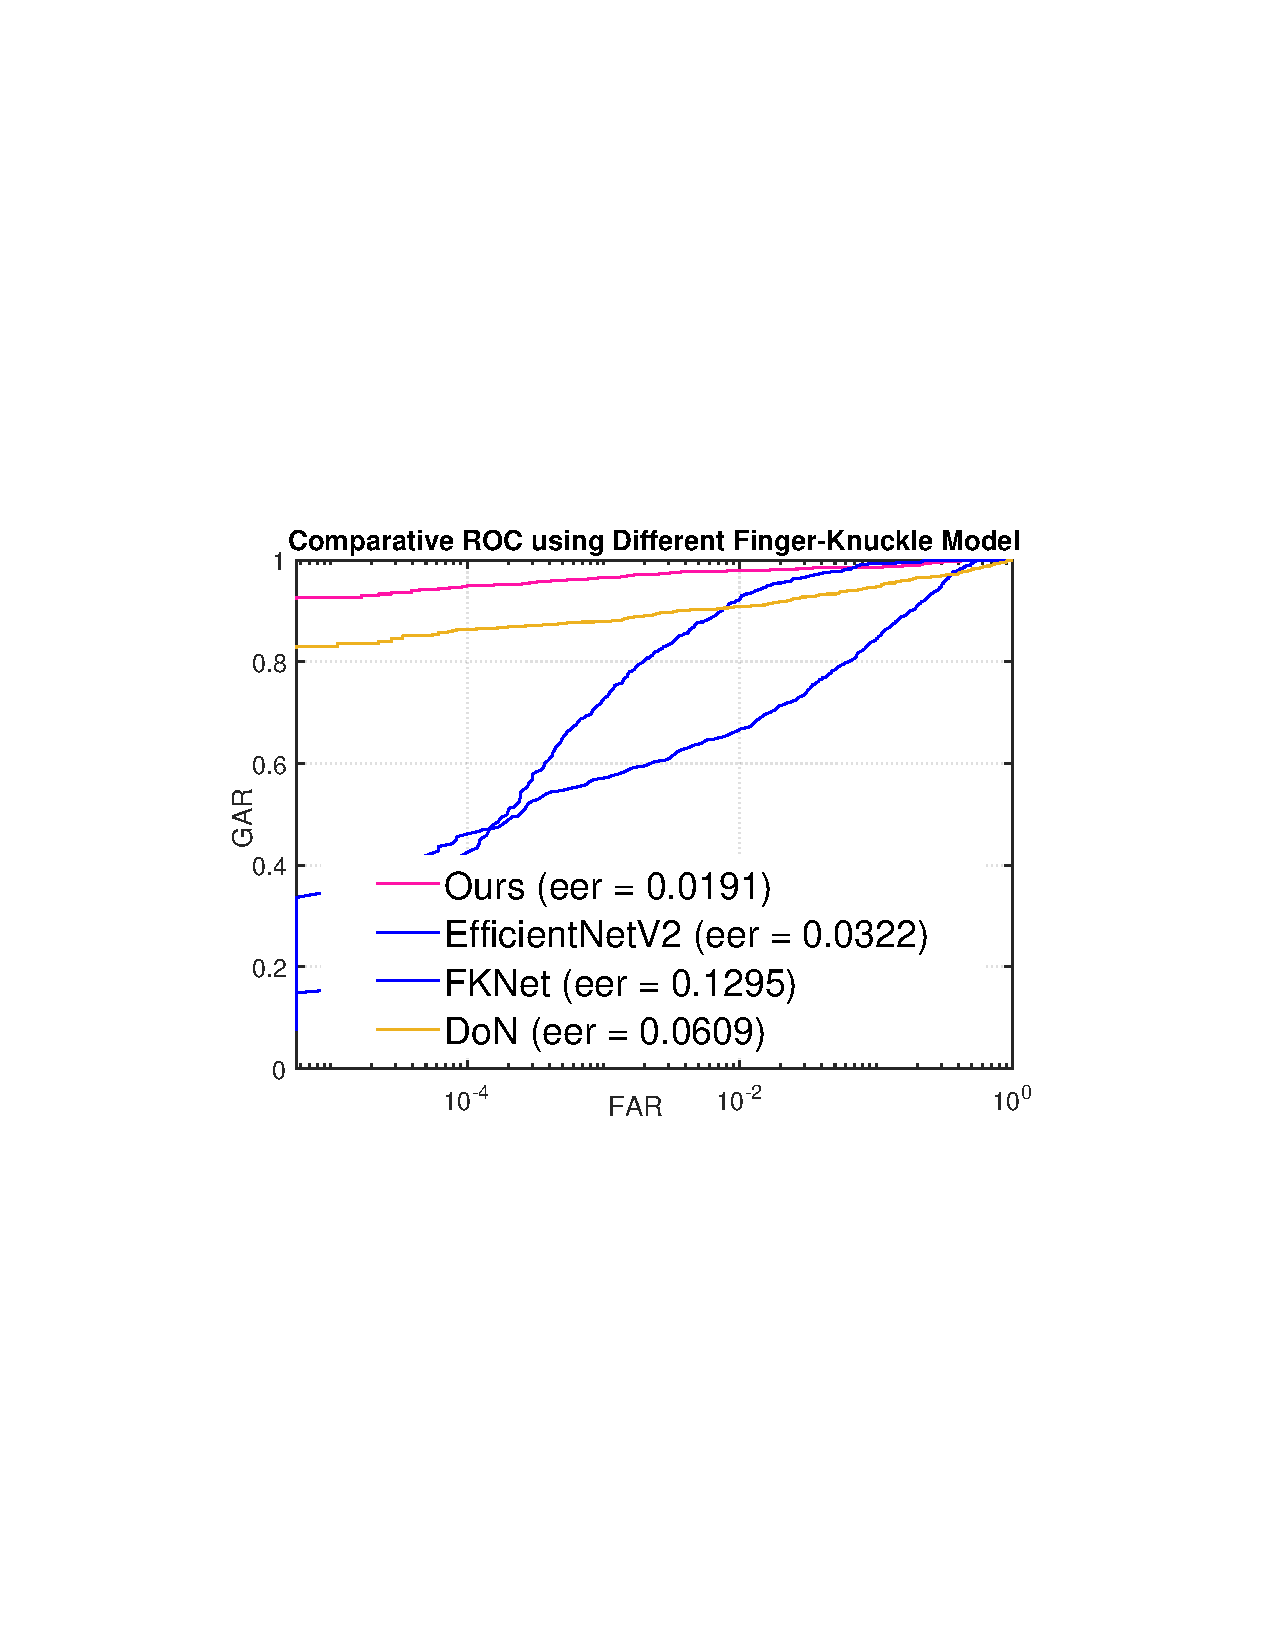
\includegraphics[width=1.7in]{Figures/fk-compare/07.pdf}
    \label{}}
    \caption{Comparative ROC using different finger knuckle model. (a) ROC of left ring finger knuckle (b) ROC of right index finger knuckle.}
    \label{compare-fingerknuckle}
\end{figure}

\section{Discussion\label{discussion}}

\textcolor{red}{Our proposal framework can get very high performance on our segmented finger knuckle in the Fig. \ref{fingerknuckle-performance}. To further demonstrate the effectiveness of our proposed framework, we also compare it with some current state-of-the-art methods, RFN \cite{liu2020contactless}, DoN \cite{zheng20163d}, FKNet \cite{cheng2020deep} and EfficientNetV2-S \cite{tan2021efficientnetv2}. Because our proposed network is based on the EfficientNetV2, we compare with it to show our method effectiveness. Firstly, all of these model are trained on the left middle finger knuckle, except the DoN model. From the Fig. \ref{compare-fingerknuckle}, our method can outperform the rest method performance, especially on the right index finger knuckle with the lowest EER value and the highest GAR value (FAR = $10^{-4}$). In terms of the EfficientNetV2-S and FKNet, both of them are classification neural network, therefore we use the feature vector before the soft-max layer to calculate similarity scores which is a drawback of classification network when predict new classes. Due to these factor, the FKNet and EfficientNetV2-S model performance is not very good performance.}

There are several fingerprint matching algorithms introduced in the literature \cite{maltoni2009handbook}. Among these the NBIS and MCC implementations are available in the public domain and were also attempted to ascertain the performance. Fig. \ref{compare-fingerprint} presents sample results from the comparative performance evaluation, with same test data and protocols as for the results in previous section. The performance from the COTS matcher was comparatively high, and therefore this matcher was employed for all the experimental results presented in previous section. 
\begin{figure}[ht]
    \centering
    \subfloat[]{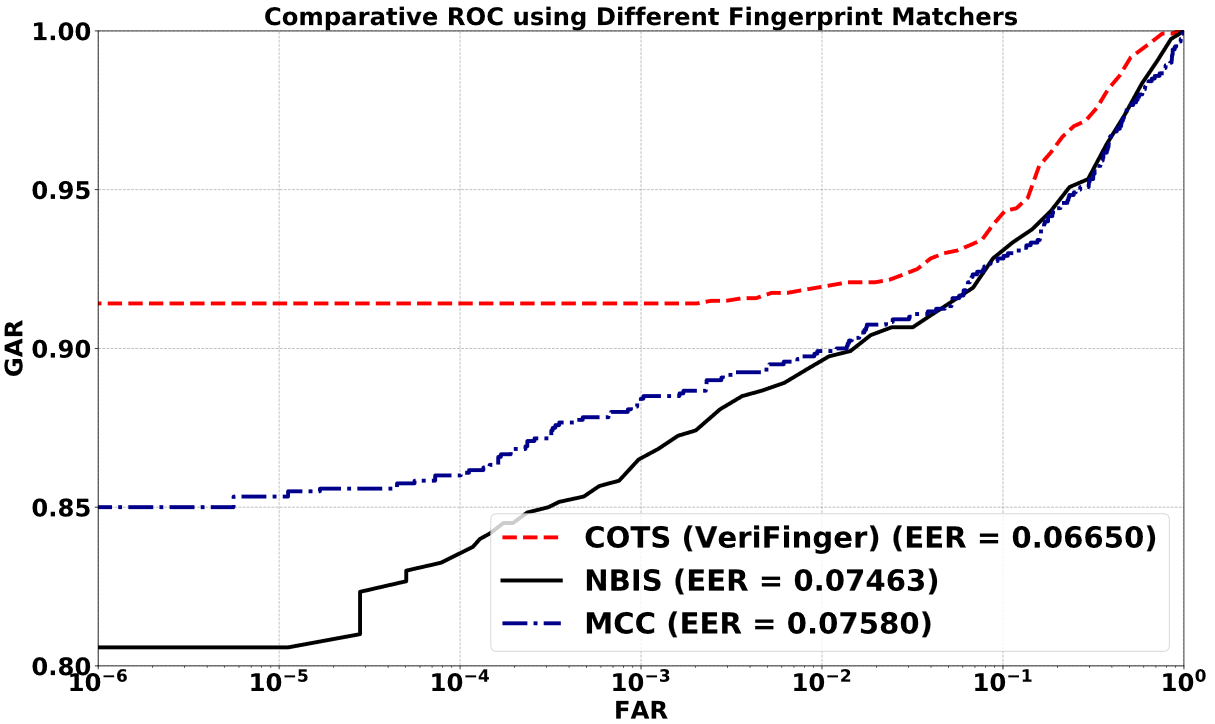
\includegraphics[width=1.6in]{Figures/compare-fingerprint-a.png}
    \label{}}
    \subfloat[]{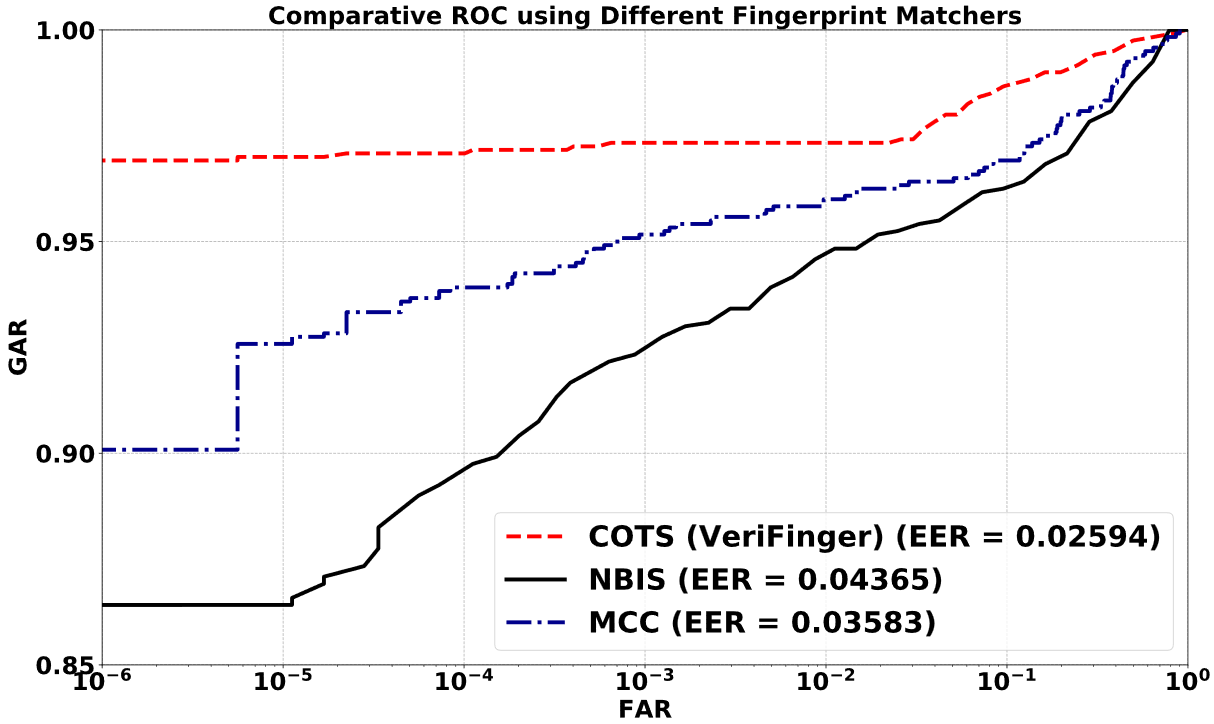
\includegraphics[width=1.6in]{Figures/compare-fingerprint-b.png}
    \label{}}
    \caption{Comparative ROC using different fingerprint matchers. (a) ROC of left ring fingerprint (b) ROC of right index fingerprint.}
    \label{compare-fingerprint}
\end{figure}

There are a range of score level combination schemes presented in the literature and can be used for the simultaneously acquired biometric samples in this work. Among these schemes, static or fixed fusion rules like sum rule, product rule, min rule, are quite attractive due to their simplicity. Therefore, we also comparatively evaluated the performance from such static score level combinations to ascertain the effectiveness of dynamic fusion introduced in this paper. Fig. \ref{compare-fusion} presents such sample comparative experimental results, with same test data and  protocols as for the results in previous section. These comparative results indicate the effectiveness of the dynamic fusion strategy to achieve more accurate performance for the simultaneously acquired fingerprint and finger knuckle images.

\begin{figure}[h]
    \centering
    \subfloat[]{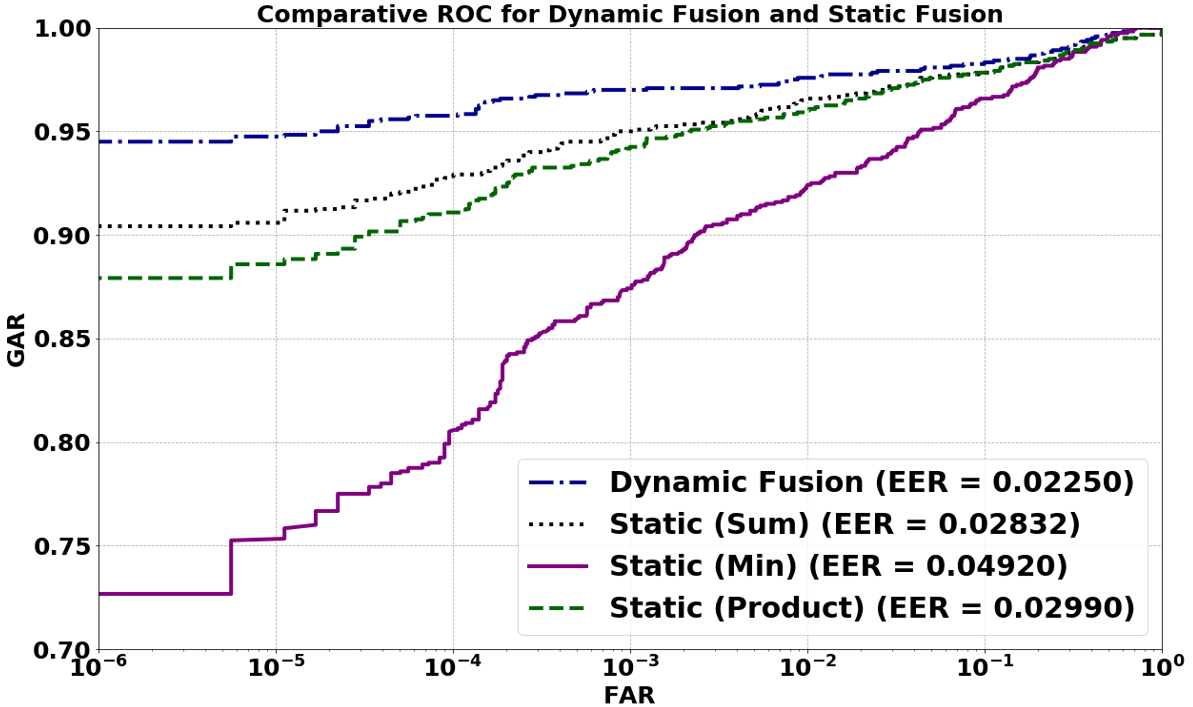
\includegraphics[width=1.6in]{Figures/compare-fusion-left.png}
    \label{}}
    \subfloat[]{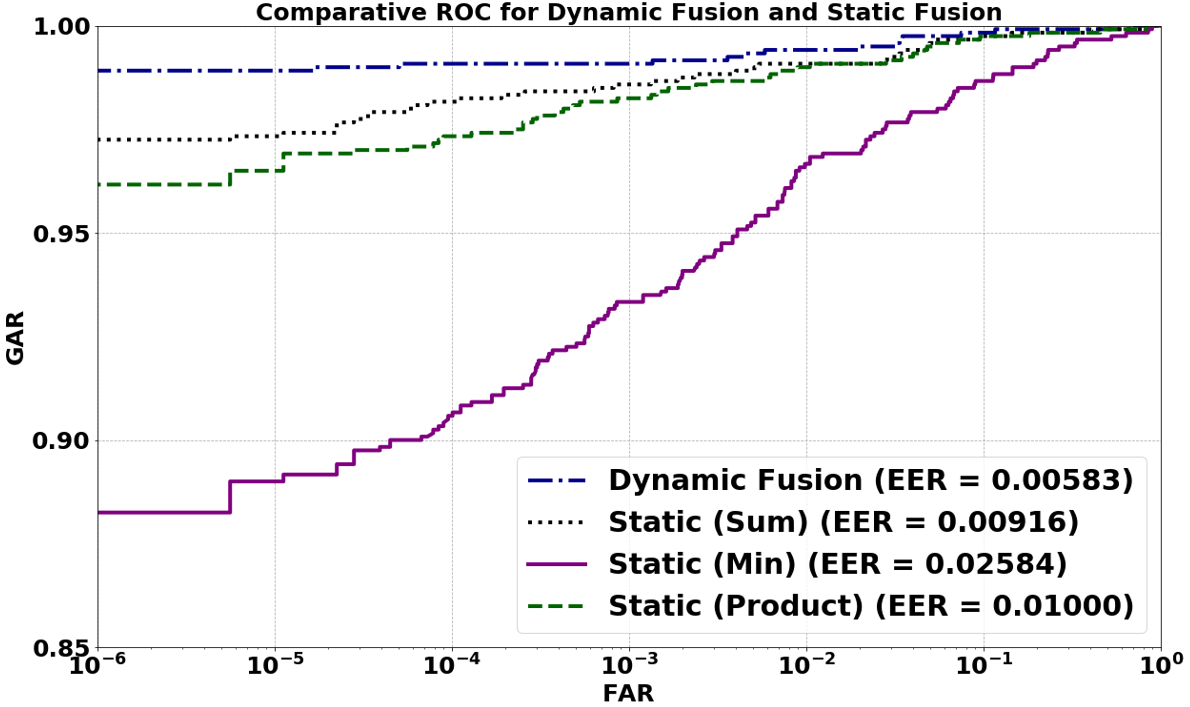
\includegraphics[width=1.6in]{Figures/compare-fusion-right.png}
    \label{}}
    \caption{Comparative ROC using different fingerprint matchers. (a) ROC of left ring fingerprint (b) ROC of right index fingerprint.}
    \label{compare-fusion}
\end{figure}

\begin{figure}[h]
    \begin{center}
    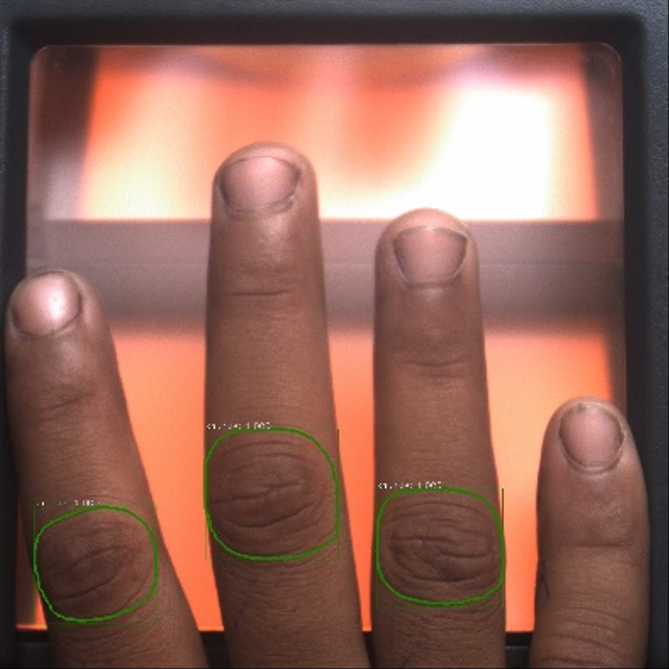
\includegraphics[width=1.1in]{Figures/failure-a.png}
    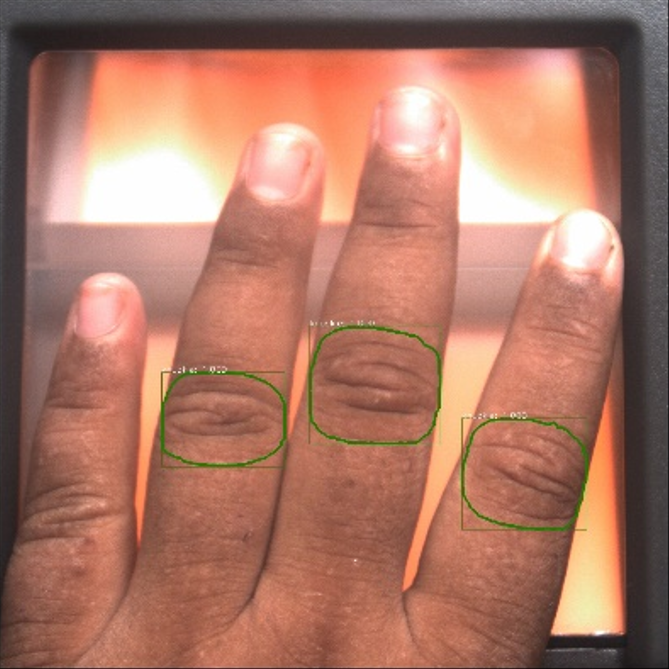
\includegraphics[width=1.1in]{Figures/failure-b.png}
    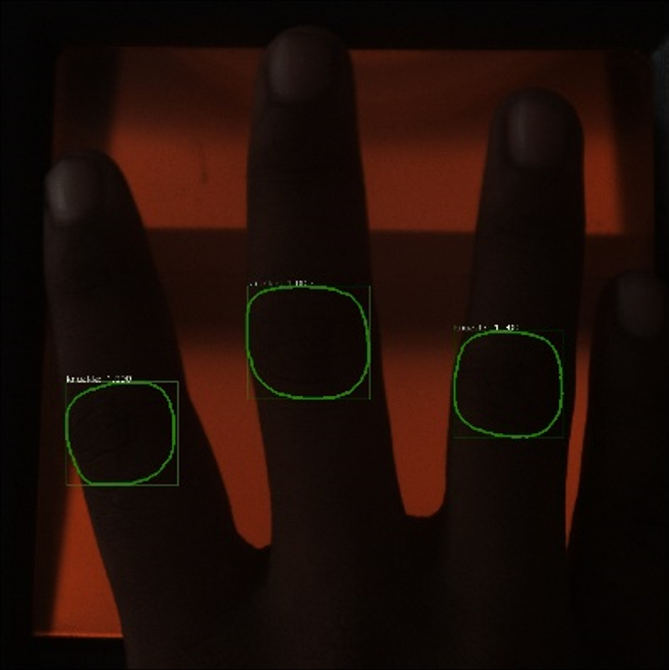
\includegraphics[width=1.1in]{Figures/failure-c.png}
    
    \hspace{0.001in}
    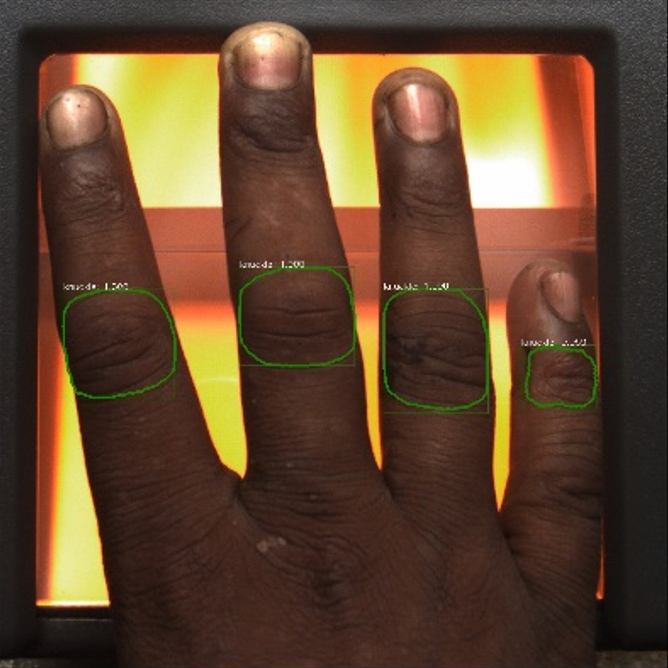
\includegraphics[width=1.1in]{Figures/failure-d.png}
    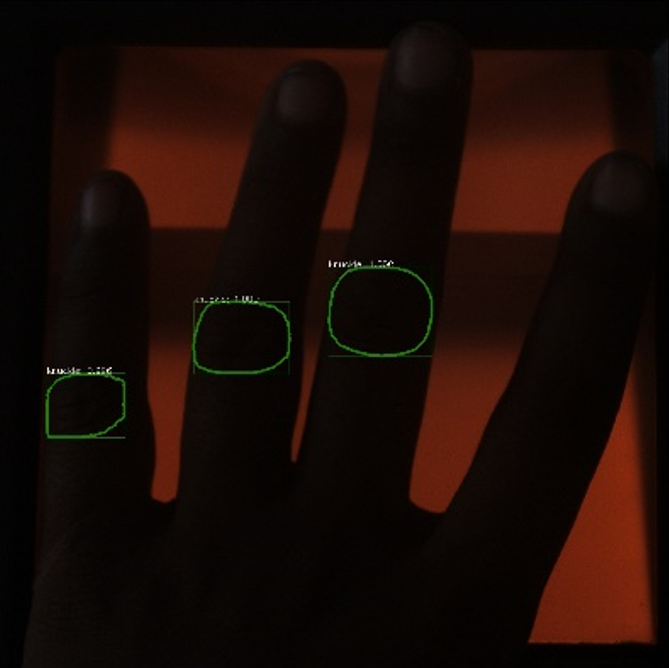
\includegraphics[width=1.1in]{Figures/failure-e.png}
    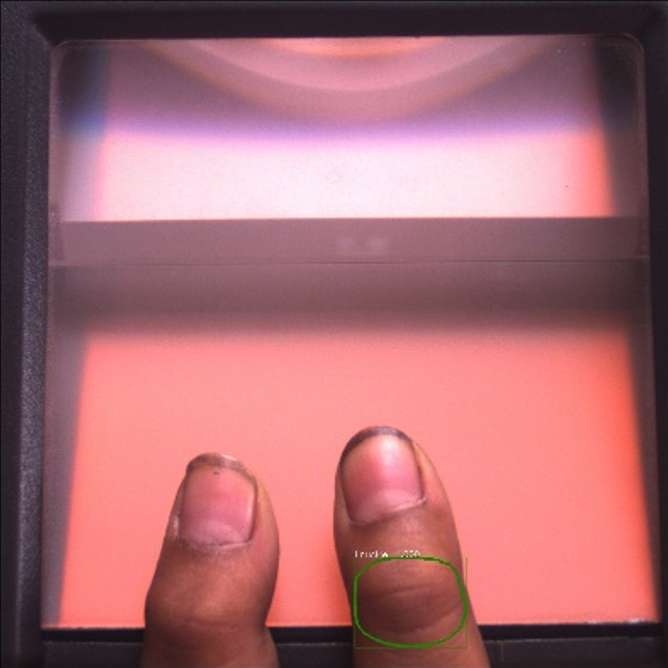
\includegraphics[width=1.1in]{Figures/failure-f.png}
    \caption{Image samples illustrating failure cases for the finger knuckle detection.}
    \label{failure-case}
    \end{center}
\end{figure}


The experimental results presented in previous section indicated the effectiveness of the simultaneously acquired finger knuckle images for the user authentication. Despite our efforts and the limited\footnote[2]{The images used to train the detector were acquired from different users and none of these subjects’ images were used for the performance evaluation presented in Section \ref{experiment}.}  availability of the images, there are many cases where the detector fails to detect the finger knuckle regions. Fig. \ref{failure-case} shows such sample failure cases for the finger knuckle detection. The first image on the left in this figure illustrates that only three finger knuckle regions are detected while the detection of finger knuckle from the little finger is not successful. The image sample in the middle indicates that the detection of finger knuckle from the left little finger is influenced by the pose of the presented finger that covers dark background of the slap fingerprint sensor. The image samples on the right side in this figure illustrates the samples that are acquired under adverse environment where the successful detection of most finger knuckle is quite encouraging. However, there are still some failure cases for the accurate detection. Such failure can be attributed not just to the availability of very limited training images but also to the limitations from the images where only partial finger knuckle regions are visible due to the presentation or the pose of presented fingers.  In many cases the knuckle regions from the thumbs are either partially imaged or not detected (e.g. last image sample in Fig. \ref{failure-fingerprint}). This is the key reason that the performance from the such finger knuckle regions is relatively low while the corresponding fingerprint performance is very high. Therefore, a separate scheme to further improve the overall match accuracy, on much larger databases as for the real applications, is required and is suggested in the further extension of this work.  

\begin{figure}
    \begin{center}
        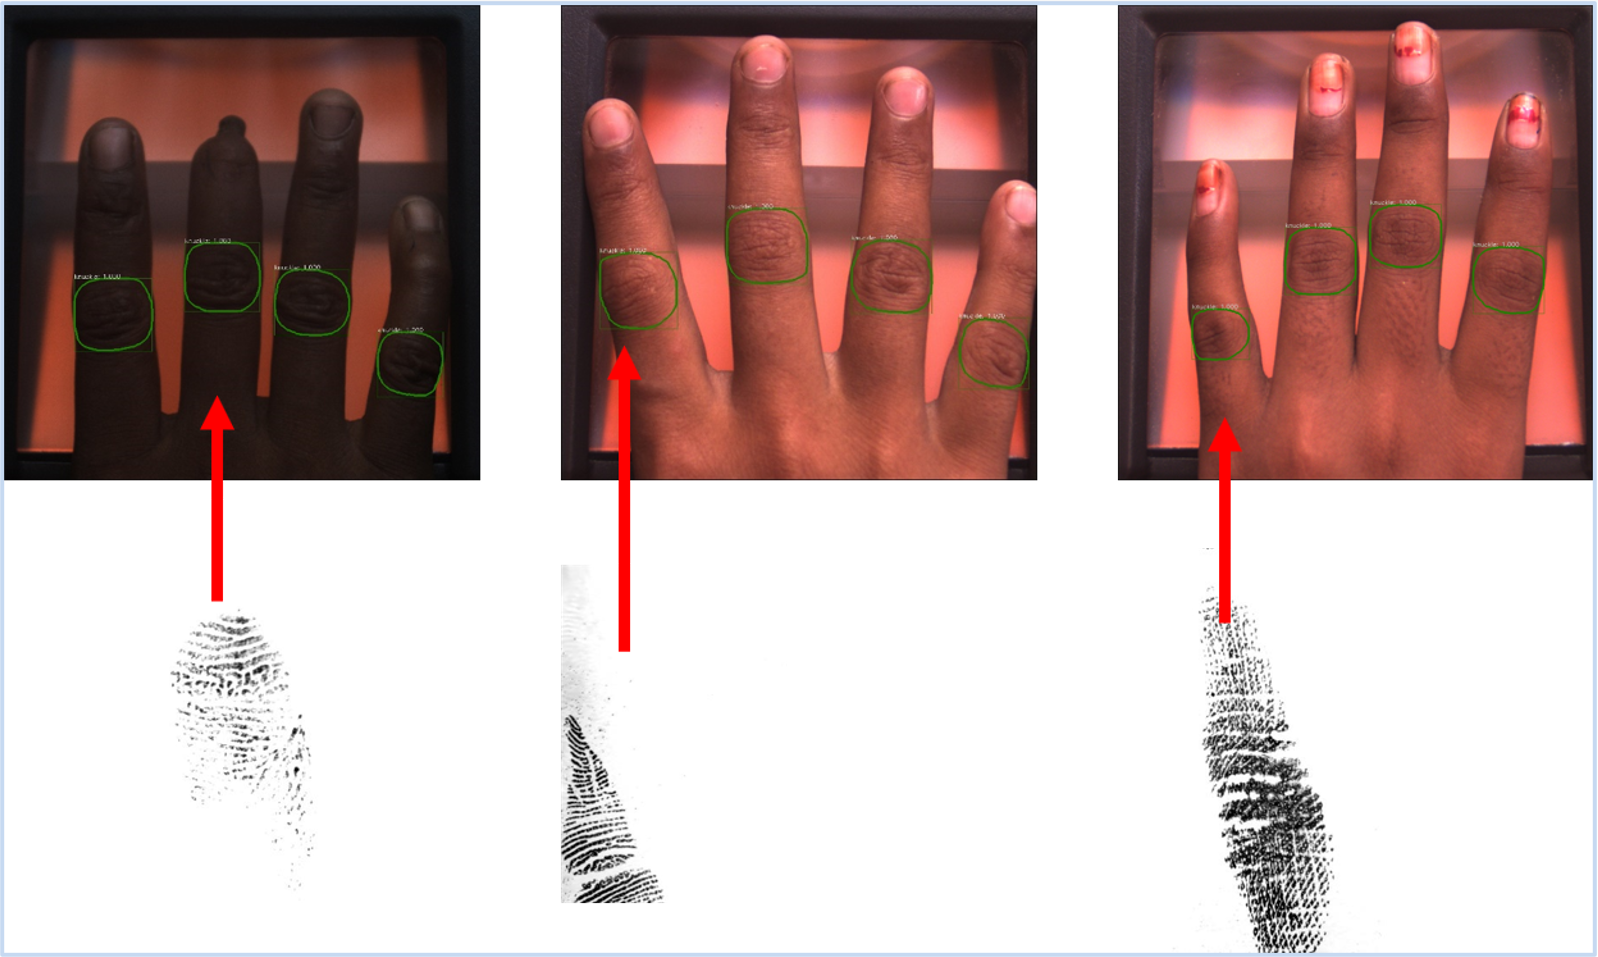
\includegraphics[width=3in]{Figures/failure-fingerprint.png}
    \end{center}
    \caption{Image samples illustrating failure cases for the fingerprint detection.}
    \label{failure-fingerprint}
\end{figure}

The fingerprint detection and the segmentation algorithms are quite matured and most commercial slap fingerprint sensors provide such implementations along with the sensor drivers. The quality of detected and segmented fingerprint images can also vary and especially for the fingerprint acquired during the real applications. These limitations were also observed during this work and there are many cases where the fingerprint region is not detected or detected images are of quite low quality. The images in Fig. \ref{failure-fingerprint} presents such failure cases for the acquired fingerprint images. The images on the first row are included to indicate the presentation of the volunteers on the slap fingerprint sensor.  The images shown in this figure on the second row illustrates the correspondingly segmented fingerprint images. The leftmost segmented image sample in this figure indicates that the middle finger fingerprint is incorrectly detected or segmented as this user has some inherent challenges with his/her fingertip. The second sample from the left indicates \textit{partial} index fingerprint segmentation and this can be largely due to the presentation of index finger which is not completely within the marked sensor surface.  Similarly, the rightmost fingerprint image sample in this figure indicated segmented fingerprint images are degraded and this can be attributed to the limitations with the pressure or the presentation fingers on the sensor surface. 